% Version 2019-01-08
% update – 161114 by Ken Arroyo Ohori: made spacing closer to Word template throughout, put proper quotes everywhere, removed spacing that could cause labels to be wrong, added non-breaking and inter-sentence spacing where applicable, removed explicit newlines
% update – 010819 by Dennis Wittich: made spacing and font size closer to Word template, updated references and refernces style
% update – 042319 by Dennis Wittich: font size of captions set to 'small', first author names are shortened, hyphenation fixed

\documentclass{isprs} % isprs class modified 23-04-2019 (Dennis Wittich)
\usepackage{subfigure}
\usepackage{setspace}
\usepackage{geometry} % added 27-02-2014 Markus Englich
\usepackage{epstopdf}
\usepackage{amsmath}
\usepackage{listings}
\usepackage[labelsep=period]{caption}  % added 14-04-2016 Markus Englich - Recommendation by Sebastian Brocks
\usepackage[british]{babel} 
\PassOptionsToPackage{hyphens}{url}\usepackage{hyperref}

\geometry{a4paper, top=25mm, left=20mm, right=20mm, bottom=25mm, headsep=10mm, footskip=12mm} % added 27-02-2014 Markus Englich
%\usepackage{enumitem}

%\usepackage{isprs}
%\usepackage[perpage,para,symbol*]{footmisc}

%\renewcommand*{\thefootnote}{\fnsymbol{footnote}}
\captionsetup{justification=centering,font=normal} % thanks to Niclas Borlin 05-05-2016
\captionsetup[figure]{font=small} % added 23-04-2019 Dennis Wittich
\captionsetup[table]{font=small} % added 23-04-2019 Dennis Wittich

\begin{document}

\title{CRYPTO-SPATIAL : AN OPEN STANDARDS SMART CONTRACTS LIBRARY FOR BUILDING GEOSPATIALLY ENABLED DECENTRALIZED APPLICATIONS ON THE ETHEREUM BLOCKCHAIN}

% KAO: Remove extra spacing
\author{
 BENAHMED DAHO Ali\textsuperscript{1}
}

% KAO: Remove extra newline
\address{
	\textsuperscript{1 }Geodetic Sciences and Topographic Works Engineer, Ain Temouchent, Algeria - bidandou@yahoo.fr\\
}

% If the corresponding author is NOT the final author, always add a % space before the subsequent comma, i.e.
% first author name\textsuperscript{a,}\thanks{Corresponding author} , % second author name \textsuperscript{b}, etc.
% thanks to Niclas Borlin 05-05-2016


\commission{VI, }{VI} %This field is optional.
\workinggroup{VI/6} %This field is optional.
\icwg{}   %This field is optional.

% KAO: Use times symbol
\abstract{
Blockchain is an emerging immature technology that disrupt many well established industries nowadays, like finance, supply chain, transportation, energy,  official registries (identity, vehicules, ...). In this contribution we present a smart contracts library, named Crypto-Spatial, written for the Ethereum Blockchain and designed to serve as a framework for geospatially enabled decentralized applications (dApps) developement. The main goal of this work is to investigate the suitability of Blockchain technology for the storge, retrieval and processing of vector geospatial data. The design and the proof-of-concept implementation presented are both based on the Open Geospatial Consortium standards, formally : Simple Feature Acces, Discrete Global Grid Systems (DGGS) and Well Known Binary (WKB). Also, the FOAM protocole concept of Crypto-Spatial Coordinate (CSC) was used to uniquely idenitify spatial features on the Blockchain immutable ledger. The desgin of the Crypto-Spatial framework was implemented as a set of smart contracts using the Solidity object oriented programming language. The implemented library was assessed toward Etheruem's best practices design patterns and known security issues (common attacks). Also, a generic architecture for geospatially enabled decentralized applications, combining blockchain and IPFS technologies, was proposed. Finally, a proof-of-concept was developped using the proposed approach which main pupose is to port the UN/FAO-SOLA  plateform to Blockchain techspace allowig more transparency and  simplifying access to users communities. The smart contracts of this prototype are live on the Rinkeby testnet and the frontend is hosted on Github pages. The source code of the work presented here is availaible on Github under Apache 2.0 licence.
}

\keywords{Ethereum Blockchain, Decentralized Applications, Smart Contracts, IPFS, OrbitDB, Land Administration, OGC Open Standards, FOAM. 
}

\maketitle

%\saythanks % added 28-02-2014 Markus Englich

\section{INTRODUCTION}\label{INTRODUCTION}
 
% KAO: Sloppy spacing ensures non-overfull lines. Can be removed if this is not an issue.
\sloppy

Geospatial technology is nowadays in the heart of major socio-economical processes giving experts and casual users valuable insights to improve there performances, optimize there daily tasks and make informed decisions. However, as for any industry sector, a growing number of deeptech technologies are emerging and disrupting well known workflows and established practices. In fact, the permeation of technologies such as IoT, Big Data Analytics, Cloud Computing, Artificial Intelligence, etc. have also greatly aided the spurt in adoption of Location Intelligence solutions \cite{geobuiz2019}. Nevertheless, we noted that in the recent years, Blockchain technology has not been intensively investigated for its suitability to leverage geospatial applications, and it's just in july 2019 that the OGC announces the creation of a new Domain Working Group for Blockchain and Distributed Ledger Technologies (BDLT/DWG) \cite{ogcbdltdwg}.

In addition, despite the existance of many initiatives to develop standardized protocols for geospatial technology on the blockchain, like \cite{foam}, \cite{xyo}, \cite{helium}, we notice that all those projects focus mainly on proof-of-location wireless networks and not on geospatial data structures and applications. To fill this gap, we investigate in this contribution the suitability of Blockchain technology for the storge, retrieval and processing of vector geospatial data. Also, a generic architecture for geospatially enabled decentralized applications, is proposed and a proof-of-concept is developped using the proposed approach.

\newpage

\section{DECENTRALIZED APPLICATIONS}\label{sec:DECENTRALIZED APPLICATIONS}
 
% KAO: Sloppy spacing ensures non-overfull lines. Can be removed if this is not an issue.
\sloppy

\subsection{Ethereum blockchain}\label{sec:Ethereum blockchain}

Ethereum blockchain can be viewed as a transaction-based state machine: we begin with a genesis state and incrementally execute transactions to morph it into some final state. It is this final state which we accept as the canonical “version” of the world of Ethereum. The state can include such information as account balances, reputations, trust arrangements, data pertaining to information of the physical world; in short, anything that can currently be represented by a computer is admissible. Transactions thus represent a valid arc between two states; the ‘valid’ part is important. A valid state transition is one which comes about through a transaction \cite{wood2014ethereum}. Formally:
\begin{equation}
\boldsymbol{\sigma}_{t+1} \equiv \Upsilon(\boldsymbol{\sigma}_{t}, T)
\end{equation}
where $\Upsilon$ is the Ethereum state transition function. In Ethereum, $\Upsilon$, together with $\boldsymbol{\sigma}$ are considerably more powerful than any existing comparable system; $\Upsilon$ allows components to carry out arbitrary computation, while $\boldsymbol{\sigma}$ allows components to store arbitrary state between transactions.

Transactions are collated into blocks; blocks are chained together using a cryptographic hash as a means of reference. Blocks function as a journal, recording a series of transactions together with the previous block and an identifier for the final state. They also punctuate the transaction series with incentives for nodes to \textit{mine}. This incentivisation takes place as a state-transition function, adding value to a nominated account \cite{wood2014ethereum}. Formally, we expand to:
\begin{eqnarray}
\boldsymbol{\sigma}_{t+1} & \equiv & \hyperlink{Pi}{\Pi}(\boldsymbol{\sigma}_{t}, B) \\
B & \equiv & (..., (T_0, T_1, ...), ...) \\
\Pi(\boldsymbol{\sigma}, B) & \equiv & \hyperlink{Omega}{\Omega}(B, \hyperlink{Upsilon}{\Upsilon}(\Upsilon(\boldsymbol{\sigma}, T_0), T_1) ...)
\end{eqnarray}

Where \hyperlink{Omega}{$\Omega$} is the block-finalisation state transition function; \hyperlink{block}{$B$} is this block, which includes a series of transactions amongst some other components; and $\hyperlink{Pi}{\Pi}$ is the block-level state-transition function.

This is the basis of the blockchain paradigm, a model that forms the backbone of not only Ethereum, but all decentralised consensus-based transaction systems to date.

In term of implementation, there are many choices of blockchains: over 200 Bitcoin variants, Ethereum and other permissioned blockchains. To meaningfully compare them, \cite{dinh2017blockbench} identified four abstraction layers found in all of these systems. (1) The consensus layer contains protocols via which a block is considered appended to the blockchain. (2) The data layer contains the structure, content and operations on the blockchain data. (3) The execution layer includes details of the runtime environment support blockchain operations. Finally, (4) the application layer includes classes of blockchain applications. 

The Crypto-Spatial framework, described in this contribution, is designed for the Ethereum Blockchain and propose a set of smart contracts for the execution layer and a cheap geometry storage solution on IPFS for the application layer.

\subsection{IPFS and OrbitDB}\label{sec:IPFS and OrbitDB}

IPFS is a distributed file system which synthesizes successful ideas from many peer-to-peer sytems, including DHTs, BitTorrent, Git, and SFS. The contribution of IPFS is simplifying, evolving, and connecting proven techniques into a single cohesive system, greater than the sum of its parts. IPFS presents a new platform for writing and deploying applications, and a new system for distributing and versioning large data. IPFS could even evolve the web itself. IPFS is peer-to-peer; no nodes are privileged. IPFS nodes store IPFS objects in local storage. Nodes connect to each other and transfer objects. These objects represent files and other data structures \cite{benet2014ipfs}.

OrbitDB. It is a distributed, peer-to-peer database that is built on top of IPFS. OrbitDB supports various kinds of databases including key-value and log databases. This makes OrbitDB an excellent choice for the decentralized prototype  \cite{orbitdb}. 

In the solution we present in this contribution, the geometry of spatial features are stored in an OrbitDB IPFS database as OGC Well Known Binary objects for simple parsing and visualisation. The databases also have listeners implemented that triggers when the databases are replicating. Thereafter, the listeners trigger the user interface to update. This ensures that the users will always have the most recent geometry available.

\subsection{Decentralized applications developement}\label{sec:Decentralized applications developement}

Developping applications for the Blockchain is very similar to developing applications with traditional web technologies with some key differences. In fact knowing if an application need blockchain technology is as important as knowing blockchain technology itself. To do that a developer must asses its needs using the folowing key questions :

%\itemize
\begin{enumerate}
\setlength\itemsep{0em}\setlength\parskip{0em}\setlength\topsep{0em}\setlength\partopsep{0em}\setlength\parsep{0em} 
\item{Is the system defining digital reationships? if yes, Blockchain is suitable for this system.} 
\item{Should data be dynamic and auditable? if yes, Blockchain is suitable.}
\item{Should data be managed by a central authority? if yes, Blockchain is not suitable in this case.}
\item{Is the speed of the network important? if yes, Blockchain is also not suitable here.}
\end{enumerate}

The figure \ref{fig:figure_dev_workflow} illustrate the developement workflow for an Ethereum Blockchain decentralized application.

\begin{figure}[ht!]
\begin{center}
		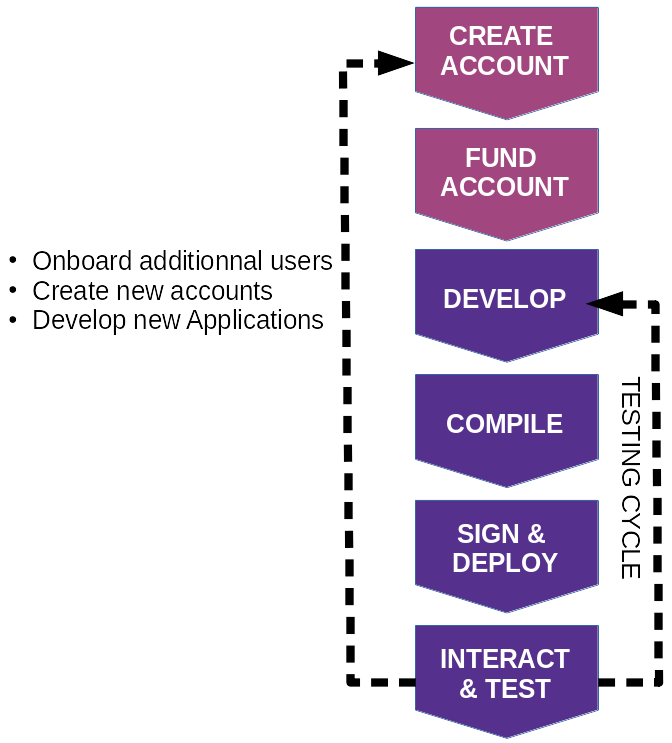
\includegraphics[width=1.0\columnwidth]{figures/eth-dev-process.png}
	\caption{Blockchain developement workflow}
\label{fig:figure_dev_workflow}
\end{center}
\end{figure}
  
The proces start by creating an account using a wallet manager like Metamask \cite{metamask} or Uport \cite{uport} and fund your account using a dedicated faucet for the selected testnet (Rinkeby, Ropsten, ...). If we develop locally we can just use ganache-cli \cite{truffle}.

As we start de developp our decentralized application we can use one of the ethereum smart contracts developpement tools like \cite{truffle}. Those tools allow us to compile, test and deploy our smart contracts on the testnet we select to use for our testing campaing before the ultimate deploiement on the Ethereum mainnet which require real Ether (cryptocurreny of Ethereum).

For the frontend, we will need a web3 library depending on the programming kanguage we use. Nevertheless, in general in the Etheruem world the ReactJS \cite{reactjs} framework is used to develop the User Interface (UI) with the web3.js \cite{web3_js} library.

\newpage

\section{THE CRYPTO-SPATIAL FRAMEWORK}\label{sec:THE CRYPTO-SPATIAL FRAMEWORK}

The Crypto-Spatial Framework is a set of smart contracts written in Solidity (object oriented programming language for Ethereum) and serves as base classes that can be specilized and customized to meet business needs. The architecture of the Crypto-Spatial smart constracts is inspired from the OGC Simple Features specifications \cite{herring2011opengis}. 

To uniquely identify spatial features on the Blockchain distributed ledger, the FOAM space concept of CryptoSpatial Coordinate (CSC) is used \cite{foamwhitepaper2018}. Nevertheless, some modifications was implemented to explore the alternatives suggested by \cite{ogcdiscuss} as the use of the H3 javascript library \cite{h3}, with an average Hexagon Edge Length  of 0.5 km (resolution 15), which it is a partially conforming implementation of the Geodesic Discrete Global Grid Systems OGC standard \cite{purss2016ogc}.

\subsection{Framework Design}\label{sec:Framework Design}

The Crypto-Spatial smart contracts library, illustrated in the following class diagram, is designed and implemented using inheritance and interfaces to simplify its resusability.

% KAO: Remove spacing before label: can cause reference to be wrong
\begin{figure}[ht!]
\begin{center}
		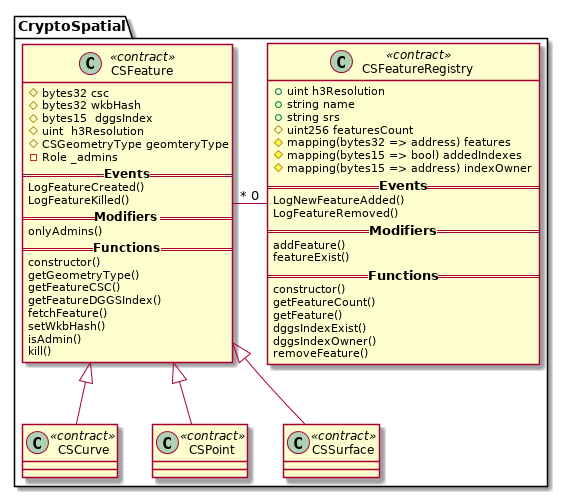
\includegraphics[width=1.0\columnwidth]{figures/class-crypto-spatial-lib.png}
	\caption{Crypto-Spatial Library Class Diagram}
\label{fig:figure_cs_lib_class}
\end{center}
\end{figure}

With this approach the developer should be able to : 

%\itemize
\begin{enumerate}
\setlength\itemsep{0em}\setlength\parskip{0em}\setlength\topsep{0em}\setlength\partopsep{0em}\setlength\parsep{0em} 
\item{inherit/use the Solidity components to build his custom contracts and develop more complex geospatial decentralized system.} 
\item{use a deployed Crypto-Spatial smart contracts and libraries that suit his business needs from ENS (ens.domains) resolvable Ethereum an addresses.}
\item{integrate/donwload the solidity reusable components (contacts) from npmjs.com and/or ethpm.com as a standalone packages or included in a widely accepted library, like openZeppelin \cite{openzeppelin}}
\item{visualize on a map all the gospatial features stored on the permanently deployed registry (as features index) to administer the features belonging to his regitries.}
\item{access a fully featured dasboard displaying all useful information about the permanently deployed features registries (the features index)}
\end{enumerate}

\subsubsection{CSFeature}\label{sec:CSFeature}

The library design, inspired from OGC Simple Features, comprises a base abstract CSFeature smart contract to represent any type of spatial features. This smart contract is specialized to hanldle Points, Curves and Surfaces with the CSPoint, CSCurve and the CSSurface smart contracts respectively.

The CSFeature smart contract includes all necessary state variables, modifiers, events and functions to store and manipulate spatial features. Main members are :

\textbf{bytes32 csc:} the Crypto-Spatial Coordinate, which is the Keccak-256 hash of the DGGS index of the spatial feature and the owner address. \\
\textbf{bytes32 wkbHash:} the Well Known Binary Hash. \\
\textbf{bytes15 dggsIndex:} the Disrcete Global Geodetic System index. \\
\textbf{uint h3Resolution:} the H3 resolution used by the registry.\\
\textbf{enum CSGeometryType:} the geometry type (Point, Curve, Surface). \\
\textbf{constructor:} the constructor that initiate all state variables. \\
\textbf{function getGeometryType:} getter for geometry type. \\
\textbf{function getFeatureCSC:} getter for CSC. \\
\textbf{function getFeatureDGGSIndex:} getter for DGGS Index. \\
\textbf{function fetchFeature:} fetch all the state variables of the spatial feature. \\
\textbf{function setWkbHash:} setter for wkbHash.\\
\textbf{function kill:} to permanently remove the spatial feature from the blockchain ledger.

\subsubsection{CSFeatureRegistry}\label{sec:CSFeatureRegistry}

The second important abstract smart contract of the Crypto-Spatial core library design is the CSFeatureRegistry which serves as the spatial features collection. 
The CSFeatureRegistry smart contract includes all necessary state variables, modifiers, events and functions to store and manipulate spatial features. The main members of this smar contracts are :

\textbf{uint h3Resolution:} the H3 resolution of the spatial feature registry (from 1 to 15) see [.....]. \\ 
\textbf{string name:} the displayed name. \\
\textbf{string srs:} the Spatial Reference System code (EPSG or equivalent). \\
\textbf{uint256 featuresCount:} the Counter of the added features. \\
\textbf{mapping features:} an addresses mapping to handle the spatial features added to the registry. \\
\textbf{mapping addedIndexes:} a boolean mapping to keep trace of added indexes. \\
\textbf{mapping indexOwner:} a mapping to keep trace of DGGS indexes owners. \\
\textbf{constructor:} the constructor that initiate all state variables. \\
\textbf{function addFeature:} a modifier that must be called by the addFeature function of inherited smart contract. \\
\textbf{function getFeatureCount:} getter of the featureCount. \\
\textbf{function getFeature:} getter for a designated spatial feature. \\
\textbf{function dggsIndexExist:} to confirm if an Index exist in the registry. \\
\textbf{function dggsIndexOwner:} returns the owner of a designated feature. \\
\textbf{function removeFeature:} permanently remove the spatial fetaure from the registry and the blockchain ledger.

\subsection{Solidity Implementation}\label{sec:Solidity Implementation}

To demonstrate the suitability of the previous design, all the smart contracts library components has been implemented in Solidity using the Truffle Suite \cite{truffle}. Herafter, a code snipet of the \textbf{addFeature} modifier demonstrating the ability to resuse business logic on the Etheruem smart contracts :

\begin{verbatim}
modifier 
addFeature(bytes15 dggsIndex, 
		   bytes32 wkbHash, 
		   address _sender) {
  require(!paused(), "Contract is paused");
  require(dggsIndex.length != 0, "Empty dggsIndex");
  require(addedIndexes[dggsIndex] == false, 
  			"DGSS Index already exist");
  require(wkbHash.length != 0, "Empty wkbHash");

  _;

  addedIndexes[dggsIndex] = true;
  indexOwner[dggsIndex] = _sender;
  bytes32 csc = CSGeometryLib.computeCSCIndex(
  				_sender, dggsIndex); 
  emit LogNewFeatureAdded(name, csc, dggsIndex, 
  				wkbHash, _sender);
  featuresCount = featuresCount.add(1);
}
\end{verbatim}

The complete implementation of the Crypto-Spatial framework can be found on the project github repository \cite{github_allilou_dela}.\\

\subsection{Security issues and design patterns}\label{sec:Security issues and design patterns}

\subsubsection{Security issues mitigation}\label{sec:Security issues mitigation}

In this section we synthetize the security vulnerabilities of Ethereum smart contracts and the vulnerabilities that can be (actually, most of them have been) exploited to carry on attacks. To avoid these common attacks a set of counter-mesures have been implemented and some of them are described below.

\textbf{Arithmetic Over/Under Flows}  To mitigate under/overflow vulnerabilities we use the openZeppelin 'SafeMath' mathematical library. 

\textbf{Reentrancy} To mitigate the reentrancy vulnerability we place any code that performs external calls after any logic updating state variables. 

Also, to avoid security vulnerabilities, the Crypto-Spatial smart contracts libray have been audited using common Ethereum security tools, formally : MythX/Mythril \cite{mythx} and Slither \cite{slihter}. All the detected vulnerabilities have been fixed.

\subsubsection{Design patterns}\label{sec:Design patterns}

As smart contracts are special immutable code executing on the Ethereum blockchain, a number of design patterns has to be applied to guarantee they are correctly prepared for all situations. This include checking the inputs as early as possible in the function body and throws an exception if the condition is not met, and restricting acces to the smart contract functions that change the states using the \cite{openzeppelin} libraries 'Ownable' and 'Roles' .

\newpage
\section{DECENTRALIZED APPLICATIONS}\label{sec:DECENTRALIZED APPLICATIONS}

Knowing that smart contracts takes only in charge the immutable part of the business logic of an application, it is also necessary to implement a frontend application to interact with the final user, set/get state variables and make calls to smart contracts functions. In the Ethereum techspace, this is generally done using ReactJS with the web3.js javascript library. To build a geospatially enabled decentralized application (GeodApp), integrating webmapping components with web3 enabled User Interface (UI) is necessary.
 
\subsection{Geospatial dApps Architecture}\label{sec:Geospatial dApps Architecture}

To build Geospatially enabed dApps for the Ethereum blockchain the following 3-tiers architecture is recommanded:

%\itemize
\begin{enumerate}
\setlength\itemsep{0em}\setlength\parskip{0em}\setlength\topsep{0em}\setlength\partopsep{0em}\setlength\parsep{0em} 
\item{The smart contracts written in Solidity.} 
\item{The IPFS/OrbitDB Storage.}
\item{The frontend web application (built with ReactJS or others).}
\end{enumerate}

The generic interaction between the previous components of a GeodApp can be described by the sequence diagram on figure [].

% KAO: Remove spacing before label: can cause reference to be wrong
\begin{figure}[ht!]
\begin{center}
		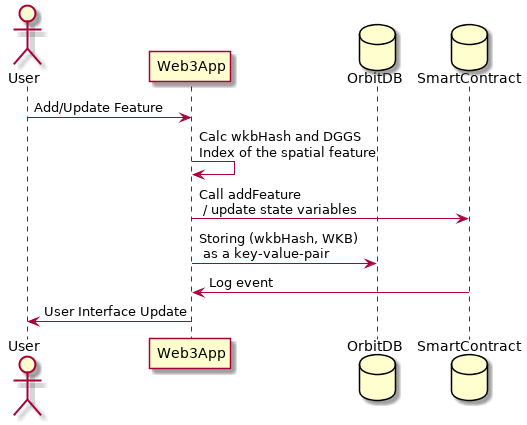
\includegraphics[width=1.0\columnwidth]{figures/seq-geospatial-dapps.png}
	\caption{Geospatial dApps sequence Diagram}
\label{fig:figure_geo_dapps_seq}
\end{center}
\end{figure}

The choice to store the geometries of the spatial features on the IPFS (OrbitDB) is justified by the gas cost of the storage on the Ethereum Blockchain. It cheaper to store the Well Known Binary (WKB) hash on the Blockchain and the WKB of the spatial feature geometry on OrbitDB/IPFS.

\subsection{Decentralized land administration (DeLA)}\label{sec:Decentralized land administration (DeLA)}

As a proof-of-concept for the proposed architecture for a Geospatial Decentrelized Application, we built DeLA GeodApp (Decentrelized Land Administration) which main objective is to implement on the Ethereum blockchain all the featires of the the open source SOLA-FAO (Solutions for Open Land Administration) \cite{sola} which is a J2EE implementation that has many uses cases in Africa and Asia. Using SOLA allows us to incorporate international best practice and standards, namely the ISO 19152:2012 standard - Geographic information — Land Administration Domain Model (LADM)) \cite{van2013iso}.

One of the major goals for porting this land registry solution to the Etherum blockchain is the ability to use it as a crowd sourcing land registry plateform \cite{seufert2013fao} to collect tenure relationships and as a tool for communities to assess and clarify their tenure regimes so to protect the individual and collective rights of their members. 

The source code of this dApp is available on \cite{dela_live} and a working version, deployed on the Rinkeby testnet, is live on \cite{github_allilou_dela}.

The class diagram on figure \ref{fig:figure_dela_class} illustrate the inheritance mecanism used the easily implement specific business logic with solidity smart contracts.

\begin{figure}[ht!]
\begin{center}
		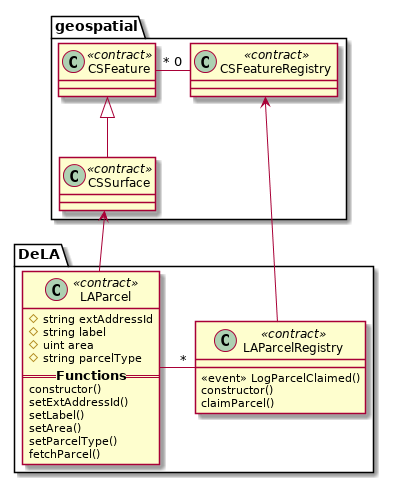
\includegraphics[width=1.0\columnwidth]{figures/class-dela.png}
	\caption{DeLA class Diagram}
\label{fig:figure_dela_class}
\end{center}
\end{figure}

To demonstrate the ability to resuse business logic on the Etheruem smart contracts, herafter a code snipet of the \textbf{claimParcel} function reusing the \textbf{CSFeature addFeature} modifier.
\begin{verbatim}
function 
claimParcel(bytes15 dggsIndex,
		bytes32 wkbHash,
		string memory extAddr,
		string memory label,
		uint area,
		string memory landUseCode,
		LAParcel.CadastralTypeCode cadastralType)
      public 
      addFeature(dggsIndex, wkbHash, msg.sender)
      returns (bytes32) {
      ...
    return csc;
  }
\end{verbatim}

\newpage

\section{BLOCKCHAIN BUSINESS MODELS}\label{sec:BLOCKCHAIN BUSINESS MODELS}

The adoption of the proof-of-concept described in this contribution can open many business opportunities as those described bellow and inspired from \cite{business_models}.

\subsection{Developement plateform}\label{sec:Developement plateform}

The main goal of Crypto-Spatial is to deliver a framework of geospatially enabled smart contracts and libraries for secure GeodApps developement. It will provide implementations of standards like OGC Simple Features Access, OGC Discrete Global Grid Systems, ISO 19107 Geographic information - Spatial schema \cite{iso2008iso} and the FOAM protocol.

The smart contracts and libraries can be deployed, as-is or extended to suit business needs, as well as Solidity components to build custom contracts and more complex decentralized systems. 

After reaching certain maturity, this framework can be submitted as a candidate to OpenZeppelin, or as an EIP (Ethereum Improvement Proposal) for standardization by the community.

\subsection{Blockchain as a service (BaaS)}\label{sec:Blockchain as a service (BaaS)}

To fully operate the DeLA platform, a set of permanently deployed components are required. In addition to the geospatially enabled smart contracts and libraries deployed on the Etheruem network (test in the developement phase and mainet after) the platform will require : 
%\itemize
\begin{enumerate}
\setlength\itemsep{0em}\setlength\parskip{0em}\setlength\topsep{0em}\setlength\partopsep{0em}\setlength\parsep{0em} 
\item{a mapping server with its geospatial database to store the spatial features (The Feature Index). The final plateform can be implemented using PostgreSQL database, PostGIS middleware and Geoserver webmapping server.} 
\item{a frontend web server to store and publish the platform Dashboard Application.}
\item{(optionnaly) a backend web server to manage business logic tasks, mainly the smart contracts events handling needed to catch the ledger recorded spatial features and populate the Features Index (database)}
\end{enumerate}

The components 1 and 3 are by design a shared services that can be easily montized for further integration in custom blockchain geospatially enabled applications, without the need to redeploy them. The deploiment diagram below illustrate this strategy.

\subsection{Blockchain based Software products}\label{sec:Blockchain based Software products}

The DeLA (Decentralized Land Administration) platform presented in this contributionis the first prototype built of a geospatially enabled application.

This prototype will serve as a fully operationnal demonstation of the proposed approach and could therefore be used in a variety of tastes, including :
%\itemize
\begin{enumerate}
\setlength\itemsep{0em}\setlength\parskip{0em}\setlength\topsep{0em}\setlength\partopsep{0em}\setlength\parsep{0em} 
\item{Permissionless/Permissioned application for governmental agencies responsible for land adminsitration and lacking critical ressources to undertake there missions as described in \cite{mckay2016voluntary}}
\item{An open data crowd sourcing plateform, OpenStreetMap like, delivering useful land parcel informations where no autoritative or commerical data are available.}
\item{A building block for specfic business case GeodApps using land information like Real estate, Investments valuation, Social responsbility, Envirmental protection, Disaster management...}
\end{enumerate}

\section{CONCLUSION}\label{sec:CONCLUSION}

In this paper we investigate the suitability of Blockchain Technology to serve as a data layer for geospatial features.We then propose an open architecture for geospatially enabled decentralized applications (GeodApps) based on Ethereum blockchain and IPFS/OrbitDB peer-to-peer storage.

The main objective of this investigation have been reached and the proposed design have been successfully implemented in a proof-of-concept GeodApp which is live on the Ethereum Rinkeby testnet and avaibale for further test and improvement as an open source project.
 
Main implications ararising from those findings are summarized on the Business models section and further works should be done to porting this solution to other type of protocoles supporting smart contracts but not using solidity, like Hyperledger fabric.


\section*{ACKNOWLEDGEMENTS}\label{ACKNOWLEDGEMENTS}

I would like to thanks Africa Blockchain Alliance to giving me the chance to enroll on the Africa Blockchain Developper Program supported by ConsenSys Academy. Also many thanks to my family members, particularly Ziad, for supporting me all the way.

{
	\begin{spacing}{1.17}
		\normalsize
		\bibliography{ISPRS2020_Submission_Daho_Blockchain} % Include your own bibliography (*.bib), style is given in isprs.cls
	\end{spacing}
}


\end{document}
¨